



\section{Storage Manager Commissioning}

% \subsection{Status, Software Schedule, and Software Organization.}

The Storage Manager project started slowly in June 2005 with just two people
from Fermilab. The number of people in the Storage Manager group doubled with time
and the first prototype was produced for the Magnet Test and Cosmic Challenge (MTCC I)
in May 2006.
During this testing it was found that the deserialization step in the Storage manager was
too slow to write out ROOT output  files thus the decision was made to write out
the binary streamer files as a temporary format for use within the Tier-0 processing.

Another lesson learned was that the Storage Manager group needed a real presence
at CERN at the experiment during data taking. The MIT group joined the Storage manager
group and strengthened the group enormously in this area. 
The MIT group took over the operations
responsibility, including the interaction with Tier-0 and the hardware.

A second prototype Storage Manager writing streamer files was produced for MTCC-II
with more optimized concurrent writing to and reading from the disk system. The event
server functionality was commissioned during MTCC-II. Remote consumers were
served by an adhoc proxy server written to run on an Apache HTTP server.
The performance goals for the Storage Manager were met in MTCC-II.

The Storage Manager group was further strengthened with additional manpower
to finish the production version for the first CMS global run exercise in May, 2007.
An additional feature request of handling DQM data in the Storage manager was
taken and completed.
A series of performance tests in joint exercises with the Tier-0 team was done early in 2007
in preparation for the May global run exercise.


The actual hardware for Phase-I of the final SM system was proposed in the Spring or 2007,
then purchased and finally delivered later that year.
The system was assembled and performance testing was begun before the end of 2007. 
In February 2008 the Tier-0 connection was commissioned.
In March a SATABeast was configured
and ``delivered'' to the DAQ group for their routine use,
i.e. both for generic DAQ system tests and CMS data taking, especially for the March Global Run.
With the  arrival of the supplementary disks (Phase-II) this two-logger-node system 
was expanded in April to consist of four  10-disk RAID5 arrays.
The latter system was used for  the CRUZET Global Run in May 2008.
Also notable for this run was the commissioning of the  SMProxyServer. 


During the 8 global run exercises conducted so far the Storage Manager goals
were met and performed well. There were of course a number of small
issues and problems during the exercises, these have been fed-back to the
software development team.
The Storage Manager team were able to respond to problems
usually in a timely manner.

In the short term future, conducting more realistic full-scale testing
is somewhat problematic from a variety of perspectives: 
the full DAQ system is not in place,
and there is considerable demand for its resources purely from among DAQ developers.
A realistic data profile and final HLT algorithms are not in place,
and the DQM related impact upon the SM is not known as it is still under development.
We see meaningful large scale system tests of the SM will increasingly be integrated
within the context of overall large scale DAQ testing.

In fact, the proposal for the CRUZET-2 global run in June are to run with a random trigger 
in addition to the cosmic trigger.
This will enable the DAQ system to be pushed to higher rates and heavier loads than
is possible with a high quality cosmic trigger. 
The unwanted random triggers will be be identified in the  HLT filter for rejection.
We propose to divert these junk events to a special stream, record them with the SM,
and even transfer them to Tier-0, where they can finally be thrown away.
This will create a more challenging data load on the SM then in the past.
We envisage supporting  CRUZET-2 of four DAQ slices with four logger nodes and two SATABeasts.



The schedule of software releases for the Storage Manager is govern by the
schedule of global run exercises and CMS Cosmic Runs (CCR) as well as
the actual start of collision data. The current schedule is to have CRUZET 2 in mid-June
and most likely another global run at zero field with the tracking system in the DAQ
before the CMS collision hall is closed for first LHC operations in mid-July.
Most of the future work for the
Storage Manager involves further commissioning of the
DQM data collection and summing, optimizing operation at the highest rates, improving
monitoring, robustness of the code and error handling. In additional documentation
of the Storage Manager will also be completed.

Installation of the hardware for the SM expansion (Sec.~\ref{sec:SMexpansion}), 
assuming a rapid procurement process, will take place by the fall.
The physical installation of the new hardware is essentially a duplicate
system in a neighboring rack, and the assembly and commissioning work
would nominally be done with no interference of the existing system.
The exception is the 4th SATABeast to be installed in the old rack,
and installation of a second Fiber Channel port on the existing PCs.
This may in fact require some reorganization of the existing rack, 
or at least presents a good opportunity to do so.
Ideally we will commission the new rack before embarking on any major
disruption of the old SM rack, but in any event, we will maintain
at least one data-ready SATABeast at all times.
Our goal is to have the entire expanded SM system operational
in early September.

The Storage Manager team resident at Fermilab will continue to do the bulk of the
software development and code maintenance work, while the MIT team will continue to
be responsible for the interaction with Tier-0 including development and maintenance of
the code related to this task, with operations, and with the
Storage Manager hardware.





\section{Storage Manager Operations}

\subsection{Routine Operations \label{sec:SMexperience}}


Throughout 2007 we supported CMS development, commissioning, and data taking
with the small provisional SM systems (\verb+cmsdisk0+ and \verb+cmsdisk1+).
This has continued in 2008, however,
since March a dual-node$+$SATABeast system has been dedicated
as the mainstay of CMS data taking.
We prefer to reserve the other two SATABeasts for technical development
and testing, but as the need arises we can quickly integrate one, or both,
of the other SATABeasts into normal CMS operations---this is essentially a matter
of small changes in configuration definitions.

As an example of the use of the SATABeast by CMS,
the data throughput for the first CRUZET Global Run in May is shown in Fig.~\ref{fig:cruzet}
for the two logger nodes.
Not surprisingly, cosmic ray running does not push the system very hard.
Operationally, once things are in place the Global Runs for the SM have
generally been smooth.
The run usually begins with a new, or even changing, software release,
and this means some setup issues are not always correct.
Once these are worked out, the SM running has been smooth except for one incident.
We began CRUZET using xfs (nodes 19 \& 20), and this seemed to caused a number
of incidents of node crashes.
Once we switched to ext3 (nodes 15 \& 16), which is most of the data, 
no further SM problems were reported.
 
% CRUZET
\begin{figure}[t]
\begin{center}  
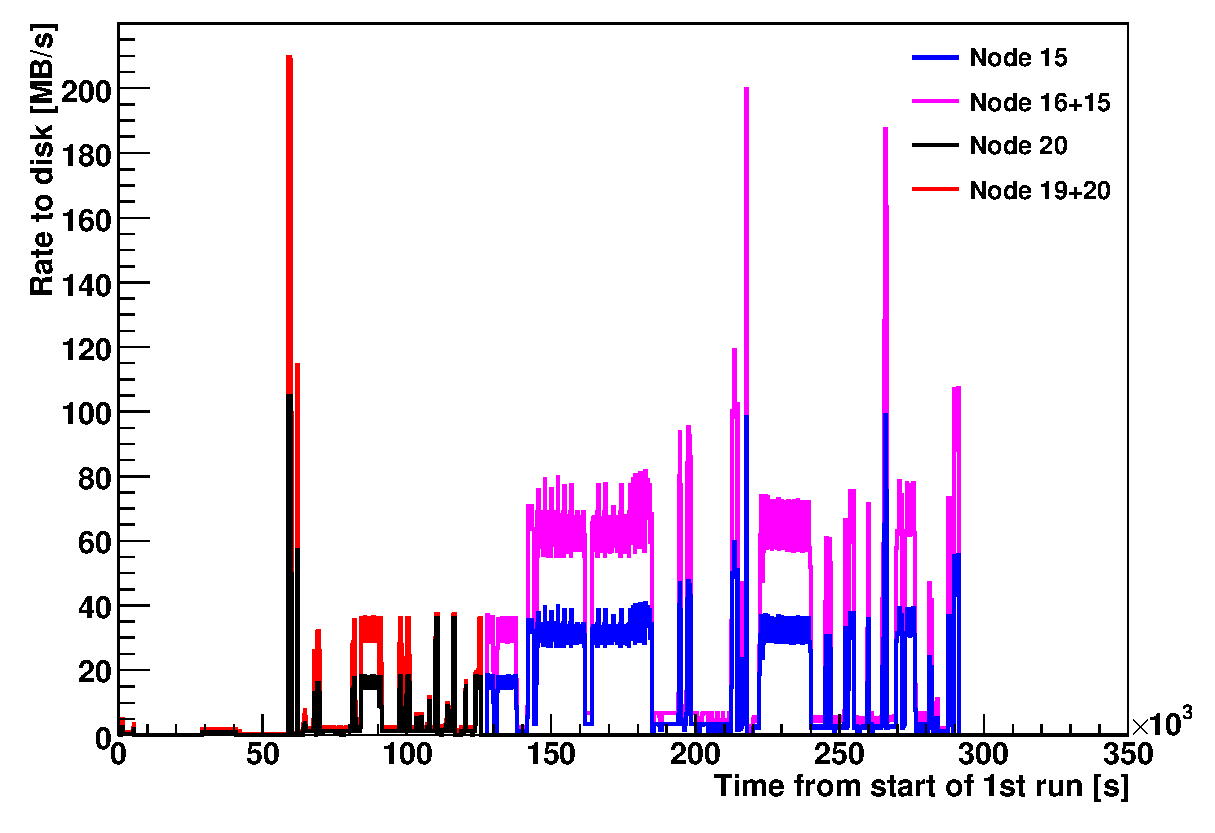
\includegraphics[width=0.9\textwidth]{Hardware/cruzetByNode}
\caption{\emph{Storage Manager throughput during the May 2008 ``CRUZET'' Global Run. 
The SM in CRUZET consisted of two logger nodes each running two SM instances,
thus making up a 4-Slice DAQ configuration; and the two logger nodes wrote
to a single SATABeast with 4 ten-disk arrays.
 The Global Run began with Nodes 19 and 20
writing to a single SATABeast with 4 disk arrays with the xfs file system.
Later in the run we switched to Nodes 15 and 16 writing to a SATABeast withh the ext3
file system.
The lower traces are the throughput of one of the two nodes
(either 15 or 20), and the upper trace is the the total through put for
the two nodes (either 15$+$16, or 19$+$21). 
The SM used only a single ``rail'' each, and thus the spikes are reaching the network 
maximum of about 220 MB/sec total throughput. The spikes are brief occurrences
due to trigger tests or improper trigger settings, 
i.e.  trigger rates for meaningful cosmics do not drive such high data rates.}}
\label{fig:cruzet}
\end{center}
\end{figure}  



\subsection{Response Plans for Hardware Failures \label{sec:SMhardfail}}

In order to minimize or avoid system down-time we envisage the following
sorts of protection against hardware failures.

\begin{itemize} 
\item {\bf Logger Node Failure:} We plan to pre-configure 2 PCs as ``warm'' spares.
The PCs would be equipped and tested with the full networking capability.
Due to the lack of spare ports for the switches, and the fact that
a preconnected spare that is truly ``hot'' will have a new identity
that would require a new DAQ configuration to be made (an expert activity),
it is deemed preferable to have ``warm'' spares which have been tested
to have full functionality, but to have them assume the host name of the
failed logger node via a Quattor system installation.
Since all DAQ PC's are administered via the Quattor management system
it is quick and easy (but still an expert action) to install a new PC with
the identity of a defunct node.
Then in addition to moving a few cables the spare node would fully assume
the old identity and be completely
functional in the existing DAQ system configuration. 

\item {\bf Fiber Channel Switch Failure:} The Fiber Channel switches have 
their own level of fall-over protection, in particular, traffic can
be rerouted to the partner switch.
However, catastrophic failures, like a complete power supply failure
can still bring down the switch.
Therefore our plan is to configure the expanded system with 2 fiber links
from each PC, one of which will be connected to each switch.
The SATABeast already has this dual connection split over the two switches.
This will then enable a complete and utter failure of a fiber channel
switch without impacting operations.
Furthermore, in the enlarged system with 4 switches in use, we plan to
pre-configure a hot spare switch which will only require moving optical
cables in order for it to take over from the failed unit.
Parenthetically, we note that this spare would also be of utility
in the event of a fiber channel switch failure in the CMS DB
installation at Cessy,  which has no spare in-hand.

\item {\bf SATABeast Controller Failure:} A part of the standard SATABeast 
design is the ability to be configured such that if one controller fails the second 
one can pickup the traffic without interruption.
We have not yet tested this feature, or seen the performance impact.
However, as each controller will only be supporting 1/16 of the data flow,
this should not have a dramatic impact.
We are investigating the particular procedures and response times
for Nexsan to provide replacement parts.

\item {\bf SATABeast Disk Failure:} The purpose, of course,
of the RAID array is that a disk may fail without loss of data.
Our baseline  mode of operation is to run RAID5 which will tolerate
a single disk failure.
Depending on the expectations of data demands, and experience with failures,
we may consider RAID6, allowing two disk failures in the same array.
With our division of four 10-disk arrays, and 2 hot spare disks,
and an assumed disk failure rate of 5\% per year, one in fact expects
to replace 2.1 disks per year per SATABeast.
In a 3-day period (eg over a weekend) there is about 1.6\% average probability
of a single disk failure out of 40 disks---assuming uncorrelated Poisson statistics,
this drops to $1.3\times 10^{-4}$ for two or more disks failing in that 3 day window
(not necessarily in the same array).
RAID5 operation seems well warranted for these average statistics.
However, as disks age this average estimate may be too optimistic,
and a more mature system in later years may warrant revisiting these numbers.

A disk failure does not lose data, but could yet impact performance.
We exercised the RAID rebuild function of the SATABeast to understand the
impact on data rates.
Rebuild times are quite substantial, and depend on array size and the rebuild 
priority setting. A small 4-disk array rebuilds in 8.4 hours for the highest
priority, and 11.1 hours in the lowest priority---all with no other activity on the SATABeast.
A 10-disk array takes 13.3 hours at the highest priority.
We started a run of the full DAQ chain to a single logger node 
to a single SATABeast array and were obtaining stable write speeds 
(no transfers or DB activity) 
of about 194 MB/sec (writing to a single array with xfs), 
and then triggered a simulated  disk failure {\it during} the run.
The write speed only decreased to 188 MB/s, but the rebuild rate dramatically increased.
Writing overlapped with the disk rebuild for about only 7 hours, after which
the array was actually filled up (there were no transfers for file removal),
but it nevertheless still almost took 22 hours to finish the rebuild.
We conclude that disk rebuilds have essentially no impact on performance,
but do take a very long time over which the array is still vulnerable.

\item {\bf Loss of Tier-0:} The connection to, and operation of, the Tier-0 center
is not our responsibility, but obviously is a potential impact.
The purpose of the large storage capacity planned for the SM was
aimed at this potential problem.
The size of the SM capacity was motivated to be able to sustain CMS data taking
through a weekend plus a day with the complete loss of Tier-0 transfers.
We presume Tier-0 services are restored within this time frame.
\end{itemize}

With the exception of the loss of a logger node, none of these failures
requires an immediate response on the part of the shift crew.
In the current DAQ setup, data taking will stop if any slice can no longer
accept events at the input, as will quickly happen if a SM node fails.
The most expedient response to a hardware loss of a logger node is
to reconfigure the DAQ to either drop the slice, 
or redistribute the traffic from the FU's of this slice.
This problem scenario is not very much different from the loss of a RU
at the beginning of the chain.
Thus reconfiguring the DAQ is a broader issue for the DAQ group.


In practice, most problems encountered are not these catastrophic hardware failures,
but smaller annoying problems arise for the shift crew like stopping executives on 
encountering of a configuration failure or general run-time failures,
We currently have been handling these problems by being experts-on-call.
In the future data-taking periods, the DAQ group will take more integrated
approach to having a generic on-call person with semi-expert knowledge to take 
care of a broad spectrum of remedial fixes.
Only after that line of defense has been exhausted would experts be called.
We have begun some documentation along these lines, but important
aspects of the system have been in flux and we most of this task
remains to be done.

\newpage

\appendix

\section{Hardware Costs and Personnel}


\subsection{Hardware Cost and Projections}
Table~\ref{tab:proto} shows the costs for the Phase-I  system purchased in 2007 
with the exception of the Logger nodes, Silicom cards and fibers, 
which where ordered together with the nodes used for the HLT farm or a database project,
and supplied by CERN. 
In total \$80k were spent on the Phase-I  system. 

A cost summary for hardware through 2010 is summarized in  Table~\ref{tab:costs}.
It includes the expenditures for 2008, which are either completed
or based on quotes supplied by vendors, except for a year old estimate 
for optical fibers.
The 2009 and 2010 projections costs are based on current costs,
with no attempt to account for falling technology prices or inflationary increases.


\begin{table}[!ht]
\begin{center}
\begin{tabular}{l|r|r}
year & cost    & product \\\hline\hline
2007 & \$66k   & 3 SATABeasts with 10 disks  \\\hline
2007 & \$6k    & 2 QLogic switches$+$hardware  \\\hline
2007 & \$8k    & 8 QLogic HBAs \\\hline
2007 & \$4k    & 2 QLogic switches hardware \\\hline
2007 & CERN    & 8 Dell PowerEdge 2950 PCs\\\hline
2007 & CERN    & 8 Silicom PEG4i \\\hline
2007 & CERN    & 20 2m fiber \\\hline\hline
\end{tabular}
\caption{Phase-I system costs.}
\label{tab:proto}
\end{center}
\end{table}

% Second Fibre Controller (2 fibre and 2 iscsi ports) Pricing $4,922
% FC switch: ~3k

\begin{table}[!ht]
\begin{center}
\begin{tabular}{l|r|r}
year  & cost      & product \\\hline\hline
2007  &     \$80k & Phase-I system \\ \hline\hline
2008~~Feb&  \$46k & 100 1TB  SATA disks  \\\hline
2008~~May& \$182k & 5 SATABeasts with 42 disks  \\
         &  \$11k & 25 Spare 1TB SATABeasts \\
         &  \$16k & 2QLogic switches$+$hardware  \\ 
         &  \$25k & 20 QLogic dual HBAs \\\hline
2008     &   \$1k & 50 2m-optical fiber \\\hline
2008     & CERN   & 10 Dell PowerEdge 2950 PCs \\\hline
\hline
2009     &  \$11k & 25 Replacement 1TB disks \\ \hline
\hline
2010     &  \$11k & 25 Replacement 1TB disks \\ \hline
2010     &   \$7k & Misc. Hardware replacement  \\  \hline
\end{tabular}
\caption{Storage Manager system costs to 2010.}
\label{tab:costs}
\end{center}
\end{table}


No new major purchases are foreseen for 2009 or 2010, 
however, warranty periods will be expiring, and in particular our original
three SATABeasts will go off warranty in 2010.
Hardware failures are of course unpredictable, but we have separated
our estimates in terms of `disks' and 'Misc. Hardware' as  statistical
projections of disk failures are more meaningful with our large sample.
The funds listed under ``Misc. Hardware replacement'' would be sufficient
for one major sub-component failure (e.g. $\sim$\$5k for SATABeast controller) and
still leave a small reserve for other small component failures.
This division is of course only conceptual, and
actual experience will dictate the ultimate allocation of funds for replacement 
hardware.

\subsection{Personnel Support for Hardware Commissioning and Operations}

At the time of the last review, in Nov 2007, the MIT hardware team 
was undergoing major personnel changes.
This centered around the then imminent departure of Markus Klute
to a faculty position, and the review committee expressed
some concerns as to the adequacy of human resources.


In late November, Research Scientist Gerry Bauer joined the SM project
full time, and PhD student Matt Rudolph joined part-time while still maintaining
activities in the tracker group.
A search was begun for a replacement of Klute, and this gap was
filled in March 2008 with the addition of Constantin Loizides,
a physicist with IT training, to the  MIT SM team. 
In early June the MIT team will be further enhanced by the addition
of Josep Serrano, an IT professional, as system administrator.
Christoph Paus continues his leadership, now as a formal USCMS 
Level-3 project co-manger along with Harry Cheung.

In summary, MIT maintained continuous personnel support of the SM hardware project 
through the departure of M. Klute, and further expanded the level of support
commensurate with the enlarged system.
We are confident that we have the necessary personnel to meet SM commitments,
and that the initial cautions expressed by the reviewers 
has been well addressed.



%% 
%% \begin{table}[!ht]
%% \begin{center}
%% \begin{tabular}{l|r|r}
%% year & cost    & product \\\hline\hline
%% 2007 & \$80k   & Phase-I  system \\\hline
%% 2008 & \$51k   & 96 SATA disks  \\\hline
%% 2009 & \$66k   & 3 SATABeasts with 10 disks  \\\hline
%% 2009 & \$51k   & 96 SATA disks  \\\hline
%% 2010 & \$17k   & Hardware replacement  \\
%% 
%% \end{tabular}
%% \caption{OLD:: Storage Manager system costs.}
%% \label{tab:costsOLD}
%% \end{center}
%% \end{table}
%% 
%% 

% memory expansion??

%% operations: 24/7 coverage plans

%% system monitoring -- faults, perform feedback, tuning...shift crew feedback

%% no requirements doc, defining divisions & boundaries ??==> sm proposal doc

%% accept amount of data can be lost?

%% disk layout on sata--a baseline

%% disaster recov?

%% interaction & misbehavior of other systems?

%% doc & proc in place before startup

%% self repairable system...

%% means of quick re-config

%% costs: add service contract --- sata replacement after 5 yr  <-- too far out 

%% Qlogic warrenty on HBA 3 yr, switches 2 yr

%% disk frag impact on writing --- very file sys dependent --- killed sys in past
